\subsection{Descrição de \textit{hardware}}\label{subsec:hardware}

Nesta Subseção, apresente as informações necessárias para se replicar o \textit{hardware} desenvolvido neste trabalho. 
Justifique suas escolhas, explicando tudo textualmente, e inclua:

\begin{itemize}
    \item Uma \textbf{lista de materiais} (BOM, do inglês \textit{bill of materials}) com os componentes necessários para a montagem do circuito~\cite{ref:bom}.
    \item Um \textbf{diagrama de blocos}, que fornece uma visão geral de como os circuitos discretos de um dispositivo ou sistema interagem. Os circuitos são representados por blocos, e suas relações são indicadas por linhas de interconexão, às vezes com setas~\cite{ref:blockdiagram}.
    \item Um ou mais \textbf{diagramas esquemáticos}, que incluem todos os componentes de um circuito, com cada componente tendo seu próprio símbolo específico~\cite{ref:esquematico}.
\end{itemize}
A Tabela \ref{tab:BOM} e as Figuras \ref{fig:exemplo_diagrama} e \ref{fig:exemplo_esquem} apresentam exemplos de uma BOM, um diagrama de blocos e um esquemático correspondentes para um circuito conversor de corrente alternada para corrente direta.


\begin{figure}[!htpb]
\centering
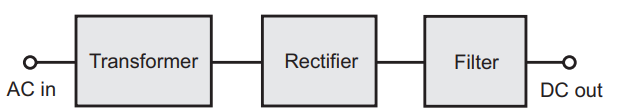
\includegraphics[width=.9\columnwidth]{figuras/Exemplo-diagrama-de-blocos.png}
\caption{Diagrama de blocos de exemplo: circuito conversor de corrente alternada para corrente direta~\cite{ref:block_n_schematic}.}
\label{fig:exemplo_diagrama}
\end{figure}

\begin{figure}[!htpb]
\centering
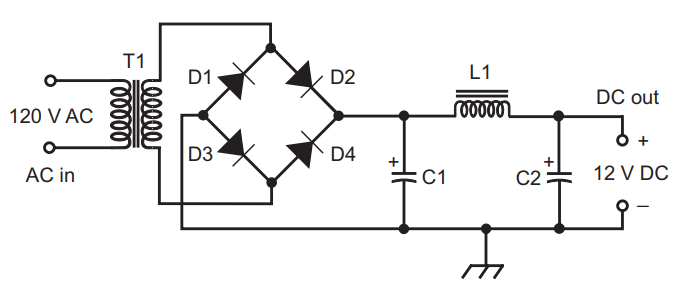
\includegraphics[width=.9\columnwidth]{figuras/Esquematico.png}
\caption{Esquemático de exemplo: circuito conversor de corrente alternada para corrente direta~\cite{ref:block_n_schematic}.}
\label{fig:exemplo_esquem}
\end{figure}


\begin{table}[!htpb]
% increase table row spacing, adjust to taste
% \renewcommand{\arraystretch}{1.3}
\caption{Lista de materiais.}
\label{tab:BOM}
\centering
\begin{tabular}{ccc}
\hline
\textbf{Componente} & \textbf{Preço unitário} & \textbf{Quantidade}\\
\hline 
Transformador INDTA1212350M 12V & R\$ 35,00 & 1 \\
Diodo 1N4007 & R\$ 1,00 & 4 \\
Capacitor eletrolítico 1 $\mu$F & R\$ 0,20 & 2\\
Indutor radial 330 $\mu$H & R\$ 1,00 & 1 \\
\hline
\textbf{Total} & R\$ 40,40 & \\
\hline
\end{tabular}
\end{table}

Tópicos importantes a serem descritos nesta Subseção incluem:

\begin{itemize}
    \item \textbf{Processamento:} RPi 3, Arduino, MSP430 etc.
    \item \textbf{Sensores:} tipos (temperatura, pressão etc.), taxas de amostragem e precisões necessárias;
    \item \textbf{Atuadores:} motores DC, relés, LEDs etc.
    \item \textbf{Comunicações:} UART, I2C, SPI, USB, WiFi, Bluetooth etc.
    \item \textbf{Armazenamento:} \textit{hard drive}, cartão SD, \textit{pendrive} etc.
    \item \textbf{Interfaces com o usuário:} botões, LEDs, display, touchscreen etc.	
    \item \textbf{Estrutura física:} formato, dimensões, posicionamento dos circuitos, dos sensores, dos atuadores e da interface com o usuário.
\end{itemize}
